% !TEX root = EnglishVocabulary.tex %指定主文件。
\ifx\collections\undefined
% !TEX program = xelatex %指定编译方式xelatex。
% !BIB program = biber %指定bib数据后台处理程序biber。
\documentclass[11pt,a4paper,UTF8,titlepage]{ctexart} %指定ctexart文档类,设置基本字号为11pt,a4大小,使用UTF-8编码保存,指定\maketitle生成单独的标题页。

\usepackage{syntonly}
%\syntaxonly %用来快速编译以排查错误,不生成DVI或PDF。
\usepackage[style=gb7714-2015]{biblatex} %调用biblatex宏包,设置参考文献样式(符合中文文献著录标准GB/T 7714-2015的样式),使用默认的后端程序biber(其支持更好,包括UTF-8等)放弃使用[backend=bibtex](只支持ascii编码)。
\addbibresource{resources/reference.bib} %加载参考文献数据库。
\usepackage{makeidx}
\makeindex %开启索引收集
\usepackage[margin=1in]{geometry} %调用geometry宏包,设置周围页边距为1英寸(为电子档设计,非打印)。
\usepackage{xcolor} %调用xcolor宏包,以支持扩展生成颜色。
\usepackage{fontspec} %调用fontspec宏包以更改西文字体族。
\setmainfont{Source Serif Pro}
\setsansfont{Source Sans Pro}
\setmonofont{Source Code Pro}
\usepackage{xeCJK} %调用xeCJK宏包以更改中文字体族。
\xeCJKsetup{AutoFakeSlant=true}  %设置xeCJK选项-伪斜体(需置于字体设置之前)。
\setCJKmainfont{思源宋体}
\setCJKsansfont{思源黑体}
\setCJKmonofont{思源等宽}
\usepackage{graphicx} %调用graphicx宏包,以支持插图。
\graphicspath{{resources/images/},{resources/images/follow/}} %加载图片路径。
\usepackage{caption} %调用caption,支持不带编号的标题。
\usepackage{wrapfig} %调用wrapfig,支持图文排版。
\usepackage{subfigure} %调用subfigure宏包进行图片图片排版。
\usepackage{tikz,tikz-qtree} %调用tikz及其扩展宏包,以支持画图。
\usepackage[subfigure]{tocloft} %tocloft与subfigure宏包冲突,不能简单调用,tocloft需设置参数。
\usepackage{tocbibind} %调用宏包以添加目录本身和参考文献进目录中。
\usepackage{multicol} %调用multicol宏包以支持多栏排版。
\usepackage[toc]{multitoc} %调用multitoc宏包,设置toc目录页,默认双栏排版。
\usepackage{enumitem} %调用emuitem,以设置列表环境。
%重订制目录命令。
\renewcommand{\tableofcontents}%
  {\chapter{\contentsname}%
  \@mkboth{\MakeUppercase\contentsname}{\MakeUppercase\contentsname}%
  \@makeschapterhead{\sourcecodename}%
  \@starttoc{toc}%
}
\usepackage{fancyhdr} %调用宏包,以设置页眉,统一格式:标题在左,页码在右。
\pagestyle{fancy}
\fancyhf{}
\fancyhead[LO]{\sffamily \rightmark}
\fancyhead[LE]{\sffamily \leftmark}
\fancyhead[ROE]{\bfseries \thepage}
%定义intro环境。
\newenvironment{intro}{\narrower\sffamily}{\par\vspace*{2ex plus 2.5ex minus 1.5ex}}
\usepackage{hyperref} %调用hyperref宏包
\hypersetup{
    colorlinks=true, %设置超链接文件带颜色
    bookmarks=true, %生成书签
    bookmarksopen=true, %书签展开
    bookmarksnumbered=true, %书签带章节编号
    CJKbookmarks=true, %cjk必设参数
    unicode, %utf-8编码必设参数
    pdftitle=标题, %设置PDF文件属性标题
    pdfauthor=Mr. Kin, %设置PDF文件属性作者
    pdfstartview=FitH %默认适合宽度显示
}

    \title{\hypertarget{title}{\textbf{标题}}}
    \addcontentsline{toc}{section}{标题页}
    \author{Written by Mr. Kin}
    \date{创建于2020.1.28,修改于\number\year.\number\month.\number\day}

\begin{document}
    \phantomsection %确保目录中的超链接指向正确的页码
    \pdfbookmark[1]{标题页}{title} %添加标题页书签
    \pagenumbering{Roman} %大写罗马样式页码
    \maketitle %生成标题页
    \pagenumbering{roman} %小写罗马样式页码
    {\centering \tableofcontents} %生成目录页
    \clearpage %新建页,分离上下两个样式页码的效果
    \pagenumbering{arabic} %阿拉伯样式页码
    \fi

    \phantomsection
    \section*{\bfseries \sffamily 关于作者}
    \addcontentsline{toc}{section}{关于作者}
    \markright{关于作者}
    
    \subsection*{\bfseries \sffamily 关于我}
    \begin{wrapfigure}[3]{L}{60pt}
       \vspace*{-20pt}
       \centering
       
\includegraphics{kin-logo}
    \end{wrapfigure}
    Mr. Kin,广东客家仁,程序猿,CG和游戏爱好者,一枚极客学生党。B站翻译up,个人up。不定时在B站直播日常:码代码,码博客,翻译,做视频,做教程。 ($\vartheta$$\bullet$\_$\bullet$)$\vartheta$ \hyperlink{follow}{\emph{(点击关注我!)}}

    \subsection*{\bfseries \sffamily 技能树}

    \begin{tikzpicture}[level distance=60pt]
        \Tree [.编程 [.C ] [.汇编 ] [.批处理 ] ]
    \end{tikzpicture}
    \qquad
    \begin{tikzpicture}[level distance=30pt]
        \Tree [.后期处理 [.开源类 [.Blender ] [.Audactiy ] [.Krita ] ] [.闭源类 [.Ps ] [.Au ] [.Pr ] ] ]   
    \end{tikzpicture}
    \qquad
    \begin{tikzpicture}[level distance=60pt]
        \Tree [.其它 [.WinOS维护 ] [.计算机拆机 ] ]
    \end{tikzpicture}

    \subsection*{\bfseries \sffamily 开源建设}

    \noindent 参与的开源软件中文化翻译

    \begin{itemize}
        \item krita文档:2018.8.5 - 2019.4.23
        \item \href{https://www.blendercn.org/5812.html?tdsourcetag=s_pctim_aiomsg}{Blender手册}:2019.7.20 - 2019.9.4 - 至今(翻译维护)
    \end{itemize}

    \subsection*{\bfseries \sffamily \hypertarget{contact}{联系方式}}

    \noindent {\small\emph{\color{red}注:联系时请注明身份,谢谢!}}

    \begin{itemize}
        \item QQ:\href{tencent://AddContact/?fromId=45&fromSubId=1&subcmd=all&uin=2312463626&website=www.oicqzone.com}{2312463626}\emph{\color{red}(点击号码即加好友)}
        \item 邮箱:2312463626@qq.com ;moyu1355@gmail.com
    \end{itemize}

    \subsection*{\bfseries \sffamily \hypertarget{follow}{关注渠道}}
    \noindent {\small\emph{\color{red}注:点击即可跳转关注!}}
    
    \begin{figure}[htbp]
        \centering
        \begin{minipage}[t]{0.21\textwidth}
            \centering
            \setlength{\abovecaptionskip}{1pt}
            \caption*{\href{https://mister-kin.github.io/}{个人博客}}
            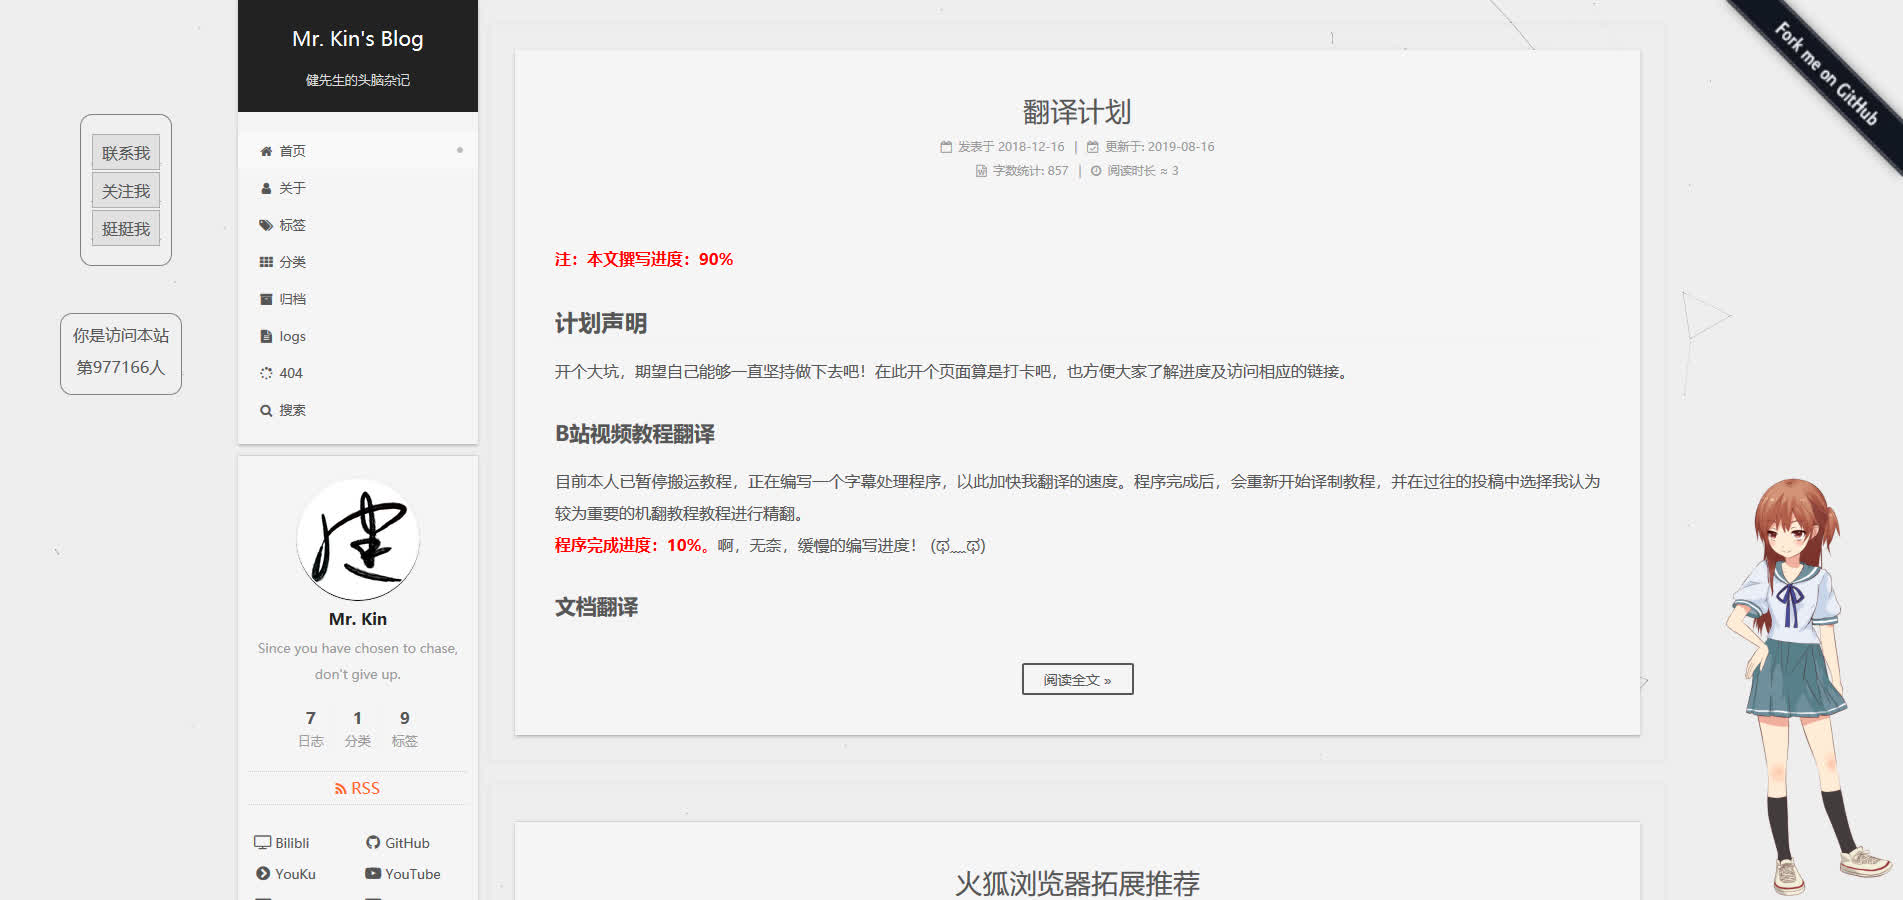
\includegraphics[scale=0.06]{follow-blog}
        \end{minipage}
        \qquad
        \begin{minipage}[t]{0.21\textwidth}
            \centering
            \setlength{\abovecaptionskip}{1pt}
            \caption*{\href{https://github.com/mister-kin}{Github}}
            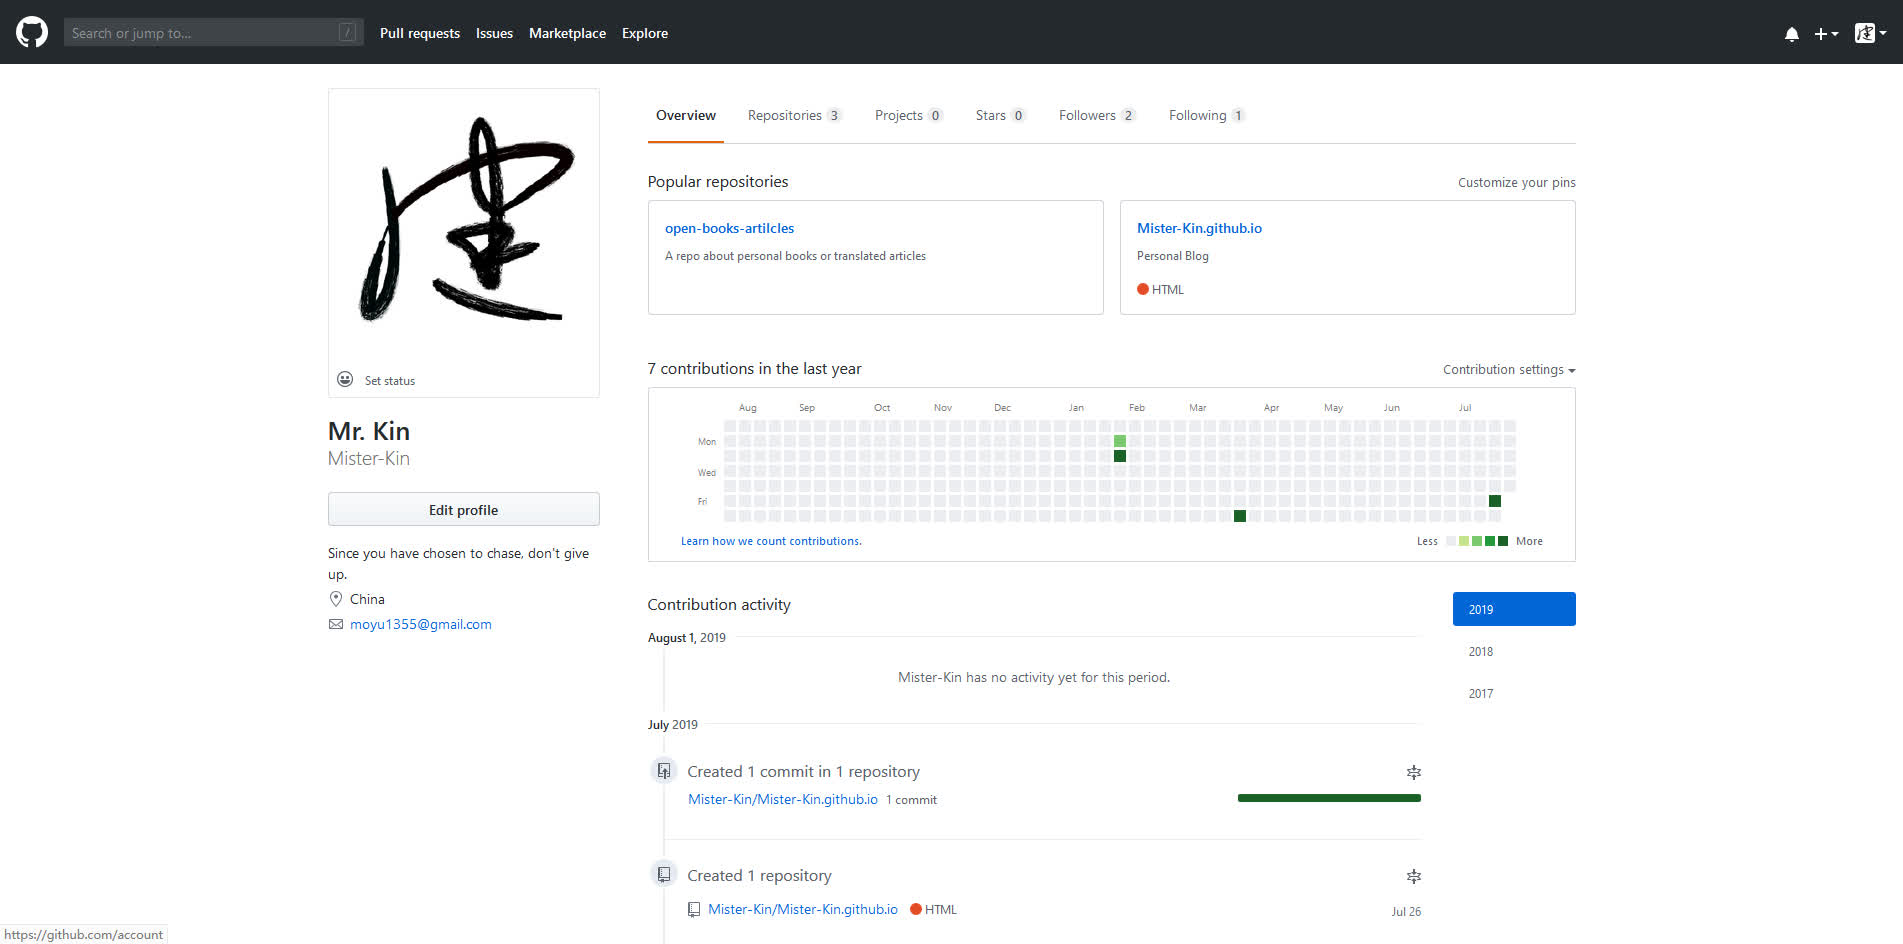
\includegraphics[scale=0.06]{follow-github}
        \end{minipage}
        \qquad
        \begin{minipage}[t]{0.21\textwidth}
            \centering
            \setlength{\abovecaptionskip}{1pt}
            \caption*{\href{https://weibo.com/6270111192/profile?topnav=1&wvr=6&is_all=1}{微博}}
            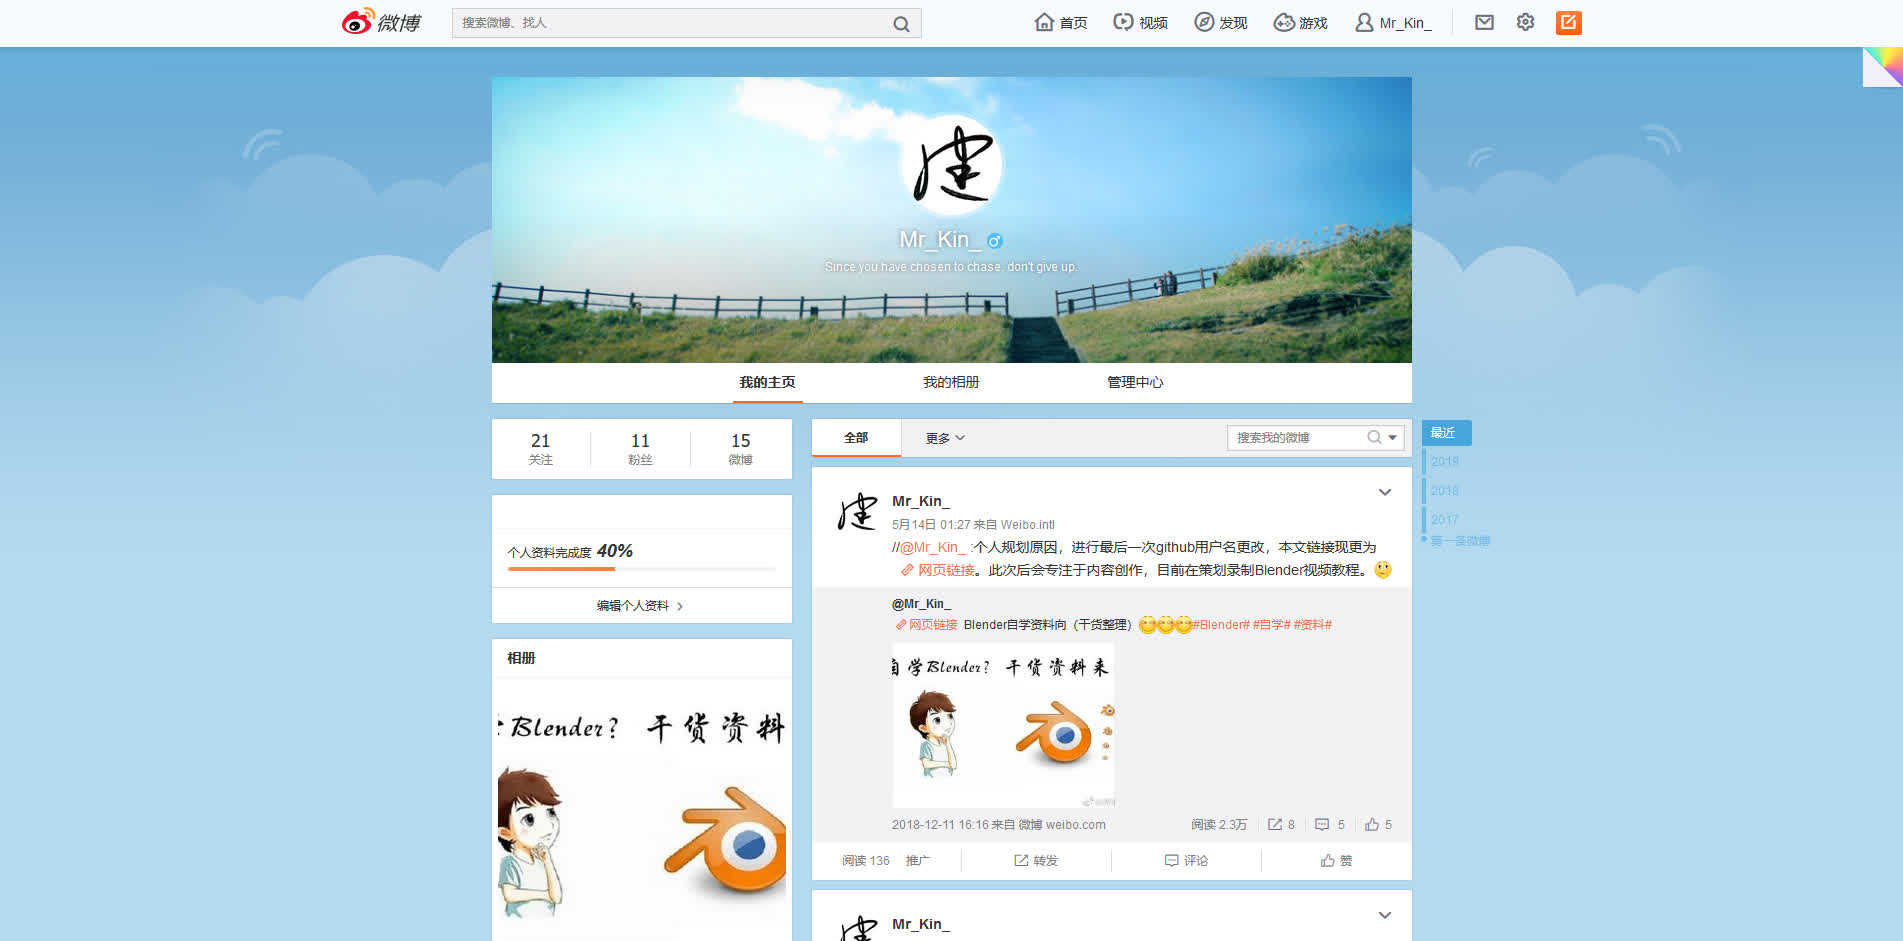
\includegraphics[scale=0.06]{follow-weibo}
        \end{minipage}
        \qquad

        \begin{minipage}[t]{0.21\textwidth}
            \centering
            \setlength{\abovecaptionskip}{1pt}
            \setlength{\belowcaptionskip}{10pt}
            \caption*{\href{http://space.bilibili.com/17025250?}{B站 - Bilibili}}
            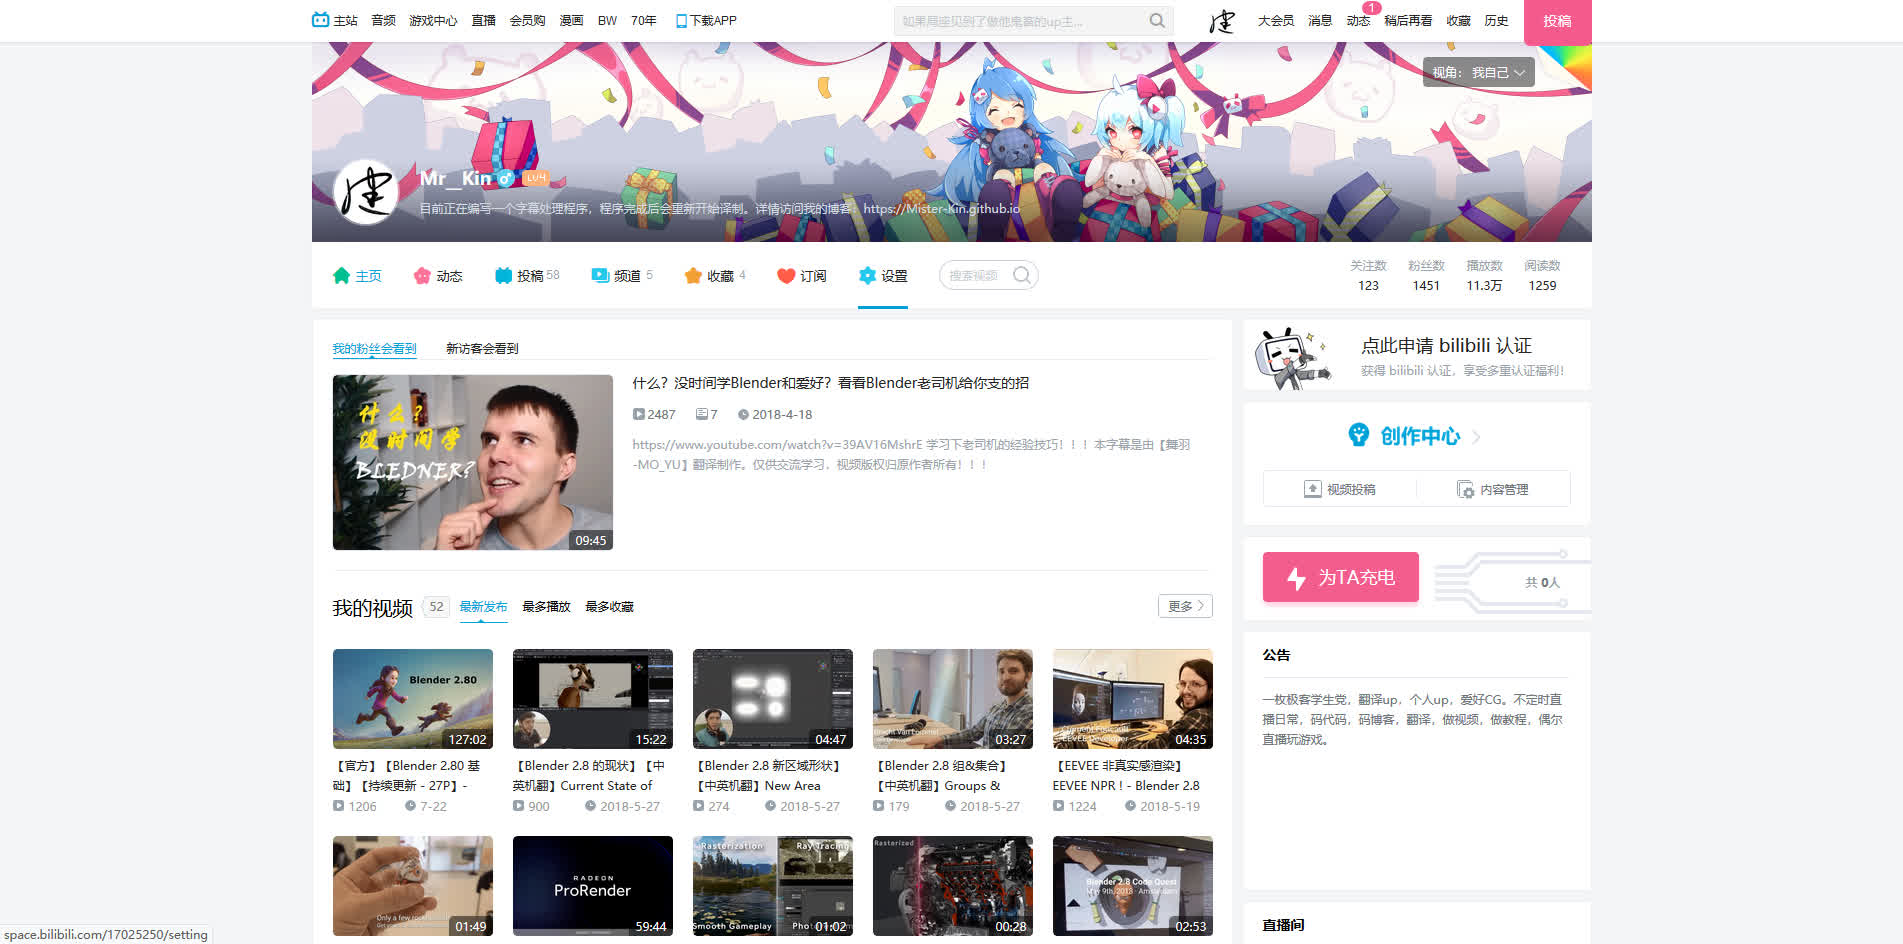
\includegraphics[scale=0.06]{follow-bilibili}
        \end{minipage}
        \qquad
        \begin{minipage}[t]{0.21\textwidth}
            \centering
            \setlength{\abovecaptionskip}{1pt}
            \setlength{\belowcaptionskip}{10pt}
            \caption*{\href{http://i.youku.com/i/UNjA3MTk5Mjgw?spm=a2hzp.8253869.0.0}{优酷}}
            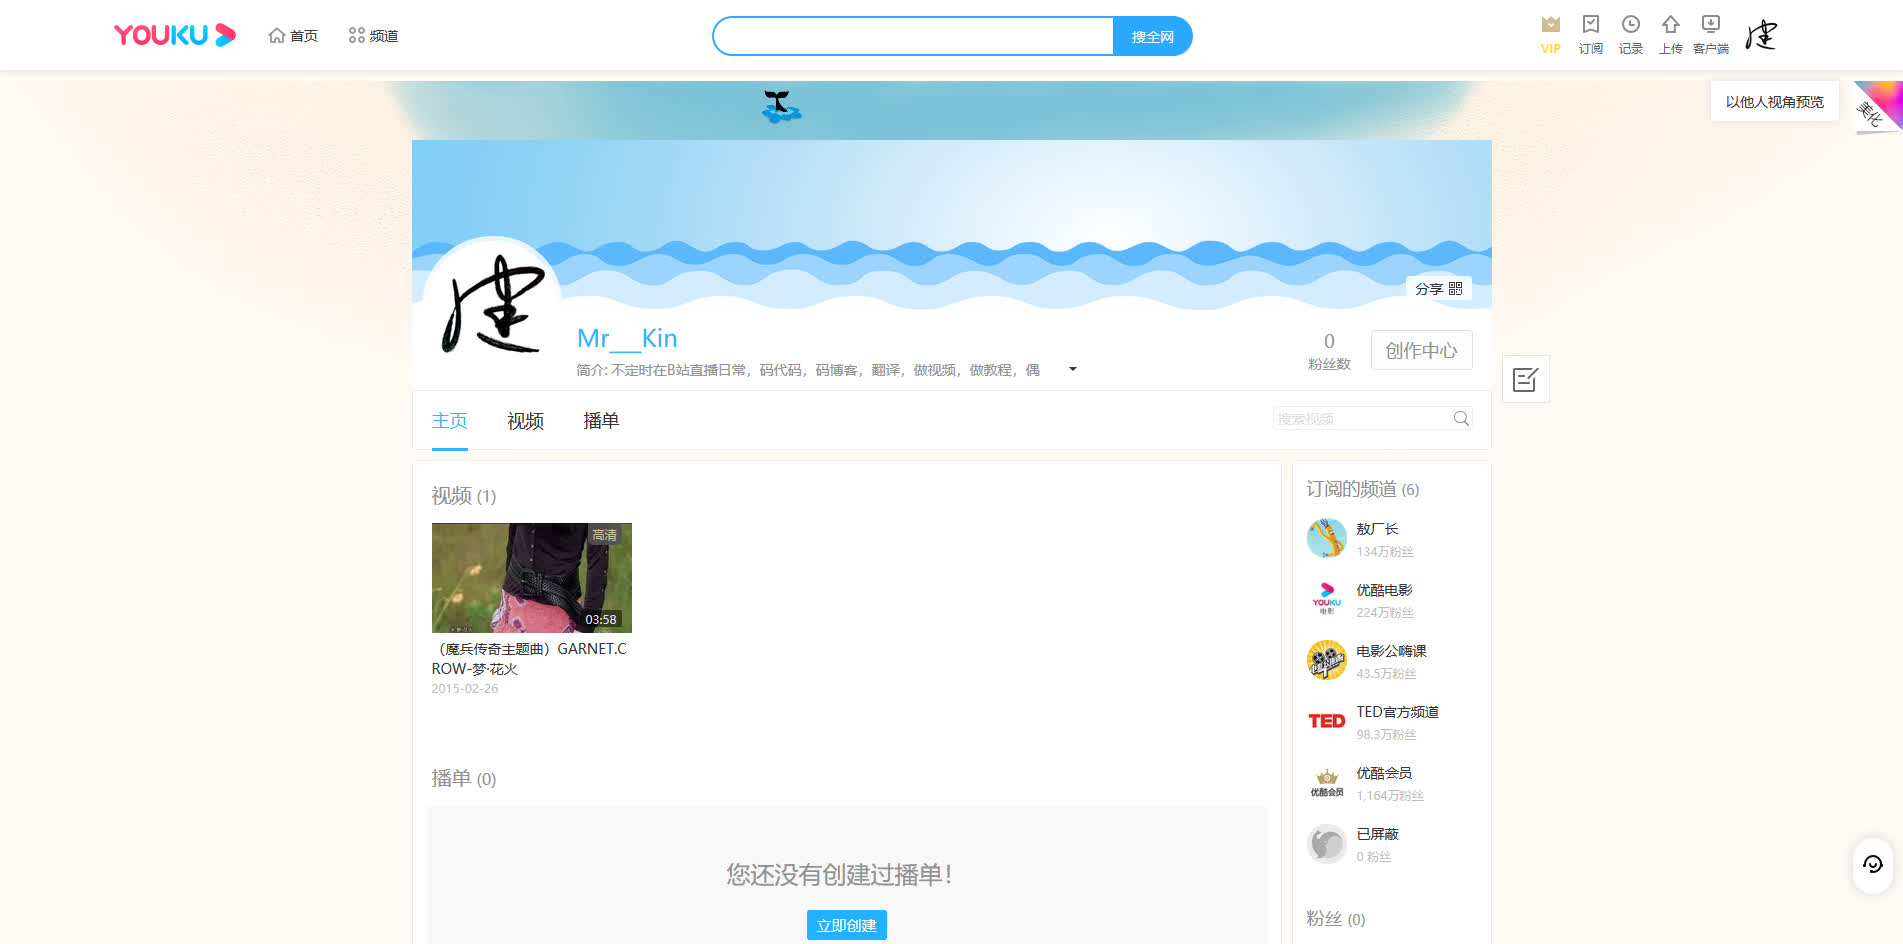
\includegraphics[scale=0.06]{follow-youku}
        \end{minipage}
        \qquad
        \begin{minipage}[t]{0.21\textwidth}
            \centering
            \setlength{\abovecaptionskip}{1pt}
            \setlength{\belowcaptionskip}{10pt}
            \caption*{\href{https://www.youtube.com/channel/UCNhtdG6whC5mlRDkrhQ0wLA?view_as=public}{油管 - Youtube}}
            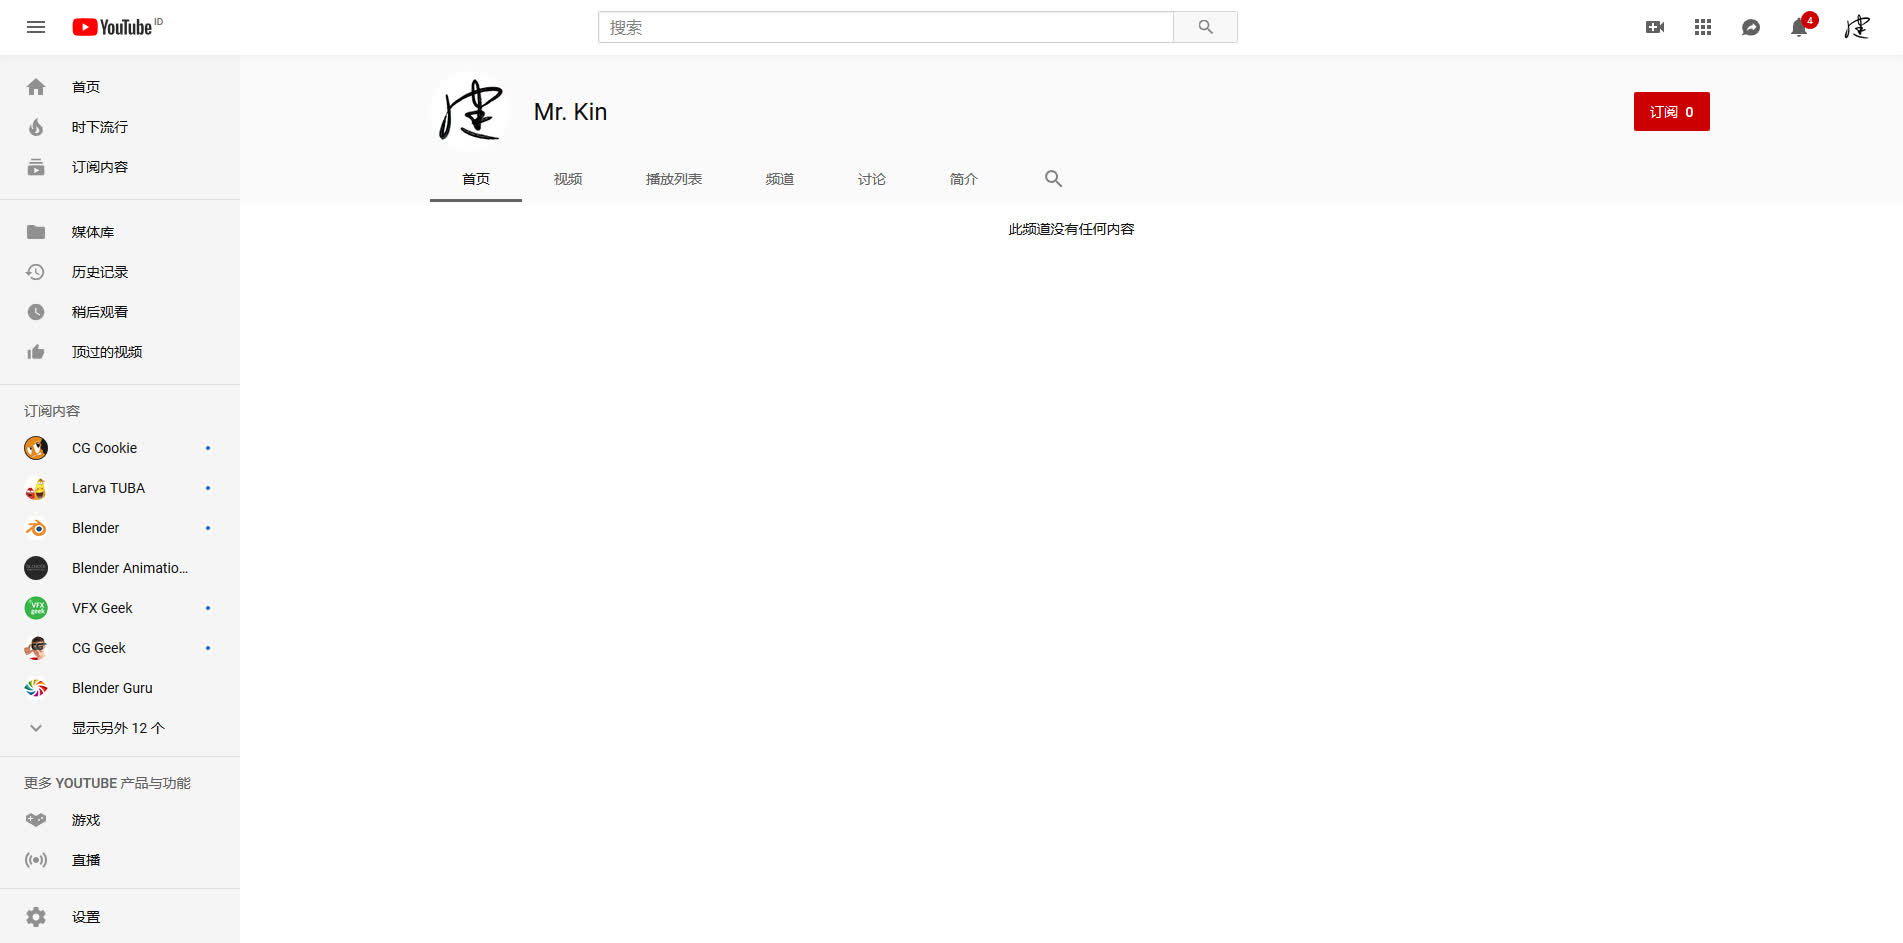
\includegraphics[scale=0.06]{follow-youtube}
        \end{minipage}
        \qquad
    \end{figure}

    \ifx\collections\undefined
    \printbibliography %生成参考文献排版。
    \addcontentsline{toc}{section}{参考文献} %添加参考文献进目录
    \clearpage %新建页,确保超链接跳转正确
    \phantomsection %确保目录中的超链接指向正确的页码
    \printindex %生成索引排版。
\end{document}
    \fi